
% --- SLIDE 2: SCULLEY'S SMALL BOX ---
\begin{frame}{The ML Code Is the Small Box}

    \centering
    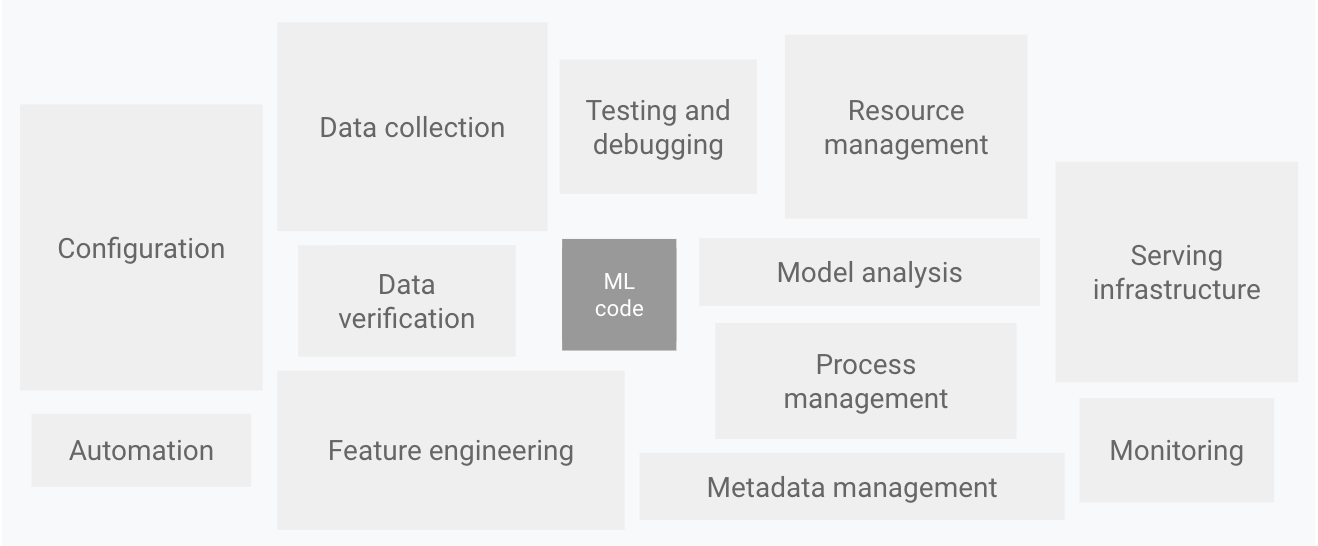
\includegraphics[width=0.92\textwidth,height=0.42\textheight,keepaspectratio]{images/mlops-foundations/gcp_elements_of_ml.png}

    {\scriptsize Source: Google Cloud, ``MLOps: Continuous delivery and automation pipelines in machine learning,''
    \href{https://cloud.google.com/architecture/mlops-continuous-delivery-and-automation-pipelines-in-machine-learning}{Cloud Architecture Center},
    Figure~1 --- after Sculley et al., \textit{Hidden Technical Debt in Machine Learning Systems}, NeurIPS 2015, Figure~1.}

    \vspace{0.6em}
    \begin{itemize}
        \item Sculley et al.\ (2015): ``\textit{Only a small fraction of real-world ML systems is composed of the ML code
              \ldots\ The required surrounding infrastructure is vast and complex.}''
        \item The grey box is what this course has been about. Everything around it is what makes it \emph{useful}.
    \end{itemize}

\end{frame}
